\documentclass[sigconf]{acmart}

\usepackage{xeCJK}
\usepackage{subfigure}
\usepackage{graphicx}
\usepackage{array}
\usepackage{enumitem}
\usepackage{multicol}
\usepackage{algorithm,algorithmic}
\usepackage{color}  
%\definecolor{shadecolor}{named}{Gray}  
\definecolor{shadecolor}{rgb}{0.92,0.92,0.92}  
\usepackage{framed}
\usepackage{ulem}

%% Font
\CJKfontspec{Noto Serif CJK TC} %思源宋體

%% ----------
\begin{document}

\title{離散數學HW10}

\author{易頡~110054809}
\orcid{}
\affiliation{%
  \institution{隨班附讀}
  \city{}
  \country{}
}

%% 刪除ACM Reference Format信息
\settopmatter{printacmref=false} % Removes citation information below abstract
\renewcommand\footnotetextcopyrightpermission[1]{} % removes footnote with conference information in first column
\pagestyle{plain} % removes running headers

\maketitle

%% ----- Question -----
\section{Question}
\begin{itemize}
	\item[-] page 683, chapter 10.1 Exercise 2
	\item[-] page 699, chapter 10.2 Exercise 8
	\item[-] page 710, chapter 10.3 Exercise 8
	\item[-] page 724, chapter 10.4 Exercise 2
	\item[-] page 741, chapter 10.5 Exercise 54
	\item[-] page 753, chapter 10.6 Exercise 26
	\item[-] page 761, chapter 10.7 Exercise 14
	\item[-] page 768, chapter 10.8 Exercise 6
\end{itemize}

%% ----- Problem -----
\section{Answer}
\subsection{page 683, chapter 10.1 Exercise 2}
\begin{shaded}
    What kind of graph (from Table 1) can be used to model a highway system between major cities where
    \begin{enumerate}[label=(\alph*)]
        \item there is an edge between the vertices representing cities if there is an interstate highway between them?
        \item there is an edge between the vertices representing cities for each interstate highway between them?
        \item there is an edge between the vertices representing cities for each interstate highway between them, and there is a loop at the vertex representing a city if there is an interstate highway that circles this city?
    \end{enumerate}
\end{shaded}
\begin{table}[h]
    \centering
	\caption{Graph Terminology.}
    \begin{tabular}{c|c|c|c}
        \hline
        $\textsl{Type}$ & $\textsl{Edges}$ & $\textsl{Multiple Edges Allowed?}$ & $\textsl{Loops Allowed?}$ \\ 
        \hline
        Simple graph & Undirected & No & No \\ 
        Multigraph & Undirected & Yes & No \\ 
        Pseudograph & Undirected & Yes & Yes \\ 
        Simple directed graph & Directed & No & No \\ 
        Directed multigraph & Directed & Yes & Yes \\ 
        Mixed graph & Directed and undirected & Yes & Yes \\ 
    	\hline
	\end{tabular}
\end{table}
\begin{enumerate}[label=(\alph*)]
    \item simple graph. Since there are no parallel edges or loops, and the edges are undirected. 
    \item \uline{~~A multigraph would in theory, be needed here. Since there may be more than one interstate highway between the same pair of cities~}
    \item \uline{~~A pseudograph is needed here, to allow for loops.~~}
\end{enumerate}

\vspace{3cm}

\subsection{page 699, chapter 10.2 Exercise 8}
\begin{shaded}
    Determine the number of vertices and edges and find the in-degree and out-degree of each vertex for the given directed multigraph.
\end{shaded}
\begin{figure}[h]
    \centering
    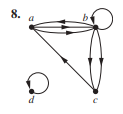
\includegraphics[width=0.25\textwidth]{10.2-8.png}
    \caption{10.2-8}
    \label{fig:a}
\end{figure}
In this directed multigraph there are \uline{~~4~~} vertices and \uline{~~8~~} edges.\\ The degrees are:\\ 
$\text{deg}^{-}(a) = 2$, $\text{deg}^{+}(a) = 2$, \\
$\text{deg}^{-}(b) = \uline{\text{~~3~~}}$, $\text{deg}^{+}(b) = \uline{\text{~~4~~}}$, \\
$\text{deg}^{-}(c) = \uline{\text{~~2~~}}$, $\text{deg}^{+}(c) = \uline{\text{~~1~~}}$, \\
$\text{deg}^{-}(d) = \uline{\text{~~1~~}}$, $\text{deg}^{+}(d) = \uline{\text{~~1~~}}$.

\clearpage

\subsection{page 710, chapter 10.3 Exercise 8}
\begin{shaded}
    Represent the graph in Exercise 4 with an adjacency matrix.
\end{shaded}
\begin{figure}[h]
    \centering
    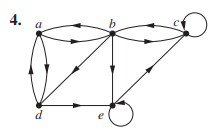
\includegraphics[width=0.35\textwidth]{10.3-8.png}
    \caption{10.3-8}
    \label{fig:b}
\end{figure}
$\begin{bmatrix}
	   0 & 1 & 0 & 1 & 0 \\
 	   1 & 0 & 1 & 1 & 1 \\
 	   0 & 1 & 1 & 0 & 0 \\
 	   1 & 0 & 0 & 0 & 1 \\
 	   0 & 0 & 1 & 0 & 1 \\
\end{bmatrix}$

\subsection{page 724, chapter 10.4 Exercise 2}
\begin{shaded}
    Does each of these lists of vertices form a path in the following graph? Which paths are simple? Which are circuits? What are the lengths of those that are paths
    \begin{enumerate}[label=(\alph*)]
        \item $a, b, e, c, b$
        \item $a, d, a, d, a$
        \item $a, d, b, e, a$
        \item $a, b, e, c, b, d, a$
    \end{enumerate}
\end{shaded}
\begin{enumerate}[label=(\alph*)]
    \item This \uline{~~is~~} (is, is not) a path of length \uline{~~4~~}, it \uline{~~is not~~} (is, is not) a circuit, it \uline{~~is~~} (is, is not) simple.
	
	\item This \uline{~~is~~} (is, is not) a path of length \uline{~~4~~}, it \uline{~~is~~} (is, is not) a circuit, it \uline{~~not~~} (is, is not) simple.

	\item This \uline{~~is not~~} (is, is not) a path, since there is no edge from d to b.

	\item This \uline{~~is not~~} (is, is not) a path, since there is no edge from b to d.
\end{enumerate}

\subsection{page 741, chapter 10.5 Exercise 54}
\begin{shaded}
    A diagnostic message can be sent out over a computer network to perform tests over all links and in all devices. What sort of paths should be used to test all links? To test all devices?
\end{shaded}
\uline{~~An Euler~~} (An Euler, A Hamilton) path will cover every link, so it can be used to test the links.\\
\uline{~~A Hamilton~~} (An Euler, A Hamilton) path will cover all the devices, so it can be used to test the devices.

\subsection{page 753, chapter 10.6 Exercise 26}
\begin{shaded}
    Solve the traveling salesperson problem for this graph by finding the total weight of all Hamilton circuits and determining a circuit with minimum total weight.
\end{shaded}
\begin{figure}[h]
    \centering
    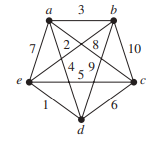
\includegraphics[width=0.35\textwidth]{10.6-26.png}
    \caption{10.6-26}
    \label{fig:c}
\end{figure}
\begin{enumerate}[label=(\alph*)]
    \item Circuit: a-b-c-d-e-a, Weight = 3 + 10 + 6 + 1 + 7 = 27
	\item Circuit: a-b-c-e-d-a, Weight = \uline{~~3 + 10 + 5 + 1 + 4 = 23~~}
	\item Circuit: a-b-d-c-e-a, Weight = \uline{~~3 + 9 + 6 + 5 + 7 = 30~~}
	\item Circuit: a-b-d-e-c-a, Weight = \uline{~~3 + 9 + 1 + 5 + 8 = 26~~}
	
	\item Circuit: a-b-e-c-d-a, Weight = \uline{~~3 + 2 + 5 + 6 + 4 = 20~~}
	\item Circuit: a-b-e-d-c-a, Weight = \uline{~~3 + 2 + 1 + 6 + 8 = 20~~}
	\item Circuit: a-c-b-d-e-a, Weight = \uline{~~8 + 10 + 9 + 1 + 7 = 35~~}
	\item Circuit: a-c-b-e-d-a, Weight = \uline{~~8 + 10 + 2 + 1 + 4 = 25~~}
	
	\item Circuit: a-c-d-b-e-a, Weight = \uline{~~8 + 6 + 9 + 2 + 7 = 32~~}
	\item Circuit: a-c-e-b-d-a, Weight = \uline{~~8 + 5 + 2 + 9 + 4 = 28~~}
	\item Circuit: a-d-b-c-e-a, Weight = \uline{~~4 + 9 + 10 + 5 + 7 = 35~~}
	\item Circuit: a-d-c-b-e-a, Weight = \uline{~~4 + 6 + 10 + 2 + 7 = 29~~}
\end{enumerate}
The circuits \uline{~~a-b-e-c-d-a~~} and \uline{~~a-b-e-d-c-a~~} are the ones with minimum total weight.

\subsection{page 761, chapter 10.7 Exercise 14}
\begin{shaded}
    Suppose that a connected planar graph has 30 edges. If a planar representation of this graph divides the plane into 20 regions, how many vertices does this graph have?
\end{shaded}
Euler's formula says that $v - e + r = 2$.\\
We are given $e = \uline{\text{~~30~~}}$ and $r = \uline{\text{~~20~~}}$. \\
Therefore $v = 2 - r + e = \uline{\text{~~2 - 20 + 30 = 12~~}}$.

\clearpage

\subsection{page 768, chapter 10.8 Exercise 6}
\begin{shaded}
    Find the chromatic number of the given graph.
\end{shaded}
\begin{figure}[h]
    \centering
    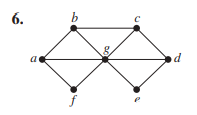
\includegraphics[width=0.35\textwidth]{10.8-6.png}
    \caption{10.8-6}
    \label{fig:d}
\end{figure}
\uline{~~Since there is a triangle, ar least 3 colors are needed. To show that 3 colors suffice, notice that we can color the vertices around the outside alternately using red and blue, and color vertex g green. a, c, e => blue, b, d, f => red, g = > green.~~}

\vspace{15cm}

\end{document}
\endinput
%%
%% End of file `sample-sigconf.tex'.
